\documentclass[12pt]{article}
\usepackage{amsmath,amstext,amsfonts,amsthm,amscd}
\usepackage{enumerate}
\usepackage[margin=1in]{geometry}
\usepackage{amsmath,amsthm,amssymb}
\usepackage{graphicx}
\usepackage{xcolor}
\usepackage[final,notref,notcite]{showkeys}
\newcommand{\N}{\mathbb{N}}
\newcommand{\Z}{\mathbb{Z}}
\newenvironment{theorem}[2][Theorem]{\begin{trivlist}
\item[\hskip \labelsep {\bfseries #1}\hskip \labelsep {\bfseries #2.}]}{\end{trivlist}}
\newenvironment{lemma}[2][Lemma]{\begin{trivlist}
\item[\hskip \labelsep {\bfseries #1}\hskip \labelsep {\bfseries #2.}]}{\end{trivlist}}
\newenvironment{exercise}[2][Exercise]{\begin{trivlist}
\item[\hskip \labelsep {\bfseries #1}\hskip \labelsep {\bfseries #2.}]}{\end{trivlist}}
\newenvironment{problem}[2][Problem]{\begin{trivlist}
\item[\hskip \labelsep {\bfseries #1}\hskip \labelsep {\bfseries #2.}]}{\end{trivlist}}
\newenvironment{question}[2][Question]{\begin{trivlist}
\item[\hskip \labelsep {\bfseries #1}\hskip \labelsep {\bfseries #2.}]}{\end{trivlist}}
\newenvironment{corollary}[2][Corollary]{\begin{trivlist}
\item[\hskip \labelsep {\bfseries #1}\hskip \labelsep {\bfseries #2.}]}{\end{trivlist}}
\newenvironment{option}[2][Option]{\begin{trivlist}
\item[\hskip \labelsep {\bfseries #1}\hskip \labelsep {\bfseries #2.}]}{\end{trivlist}}


\pagenumbering{gobble}% Remove page numbers (and reset to 1)
\clearpage
\thispagestyle{empty}
\usepackage{framed}
\title{CPS 5310 Extra Credit}
\date{}
\begin{document}
%%%%%%%%%%%%%%%%%%%%%%%%%%%%%%%%%%%%%%%%%%%%%%%%%%
\maketitle

%%%%%%%%%%%%%%%%%%%%%%%%%%%%%%%%%%%%%%%%%%%%%%%%%%%
\begin{enumerate}[{\bf I.}] 
\item (40 pts) 
 Consider the model of a vibrating rectangular membrane with tension $12.5$ lbs/ft and density $2.5$ slugs/ft$^2$ and is fixed along its entire boundary in the $xy$-plane at all times $t \in [0,T]$.
Suppose that the initial displacement is %is given by $u_0(x,y)$
\[
g(x,y)=0.1(4x-x^2)(2y- y^2) \ ft
\]
and the initial velocity is zero. Furthermore, assume that
this thin rectangular homogeneous elastic membrane is of dimension $4 \ { \text {ft}} \times \ 2$ ft and that the ground state of this membrane is described by a bounded domain $\Omega\subset \mathbb{R}^2$ with boundary $\Gamma.$ %=\partial\Omega$. % and initially  
\begin{enumerate}
\item 
Set up the partial differential equation (PDE) modeling the deflections $u(x,y,t)$ of the rectangular membrane over the time interval $[0,T]$. Make sure to specify all the boundary conditions and initial conditions.

Answer: The partial differential equation can be written as


\begin{align}
\frac{\partial^2 u}{\partial t^2} = c^2 (\frac{\partial^2 u}{\partial x^2} + \frac{\partial^2 u}{\partial y^2})
\end{align}

where $u = u(x,y,t) $ and $c^2= \frac{T}{\rho}$.

Boundary Conditions:
\begin{align}
u(0,y,t) = u(a,y,t) = 0 
\nonumber
\\  0 \leq y \leq b 
\nonumber
\\ t\geq 0
\\u(x,0,t) = u(x,b,t) = 0 
\nonumber
\\  0 \leq x \leq a 
\nonumber
\\ t\geq 0
\end{align}

Initial Conditions:
\begin{align}
u(x,y,t = 0) = g(x,y) =0.1(4x -x^2)(2y -y^2)ft
\\ \frac{\partial u(x,y,t)}{\partial t}|_t_=_0 = v(x,y)   
\end{align}

where $(x,y) \subset R$



\item Find the deflection $u(x,y,t)$ of the rectangular membrane at any point $(x,y)$ of the membrane and at any time $t$.  



 Answer:
 
 Using the separation of variables, we can write the generalized form of the solution as 
 \begin{align}
 \nonumber
 u(x,y,t) = X(x)Y(x)T(t)
 \\ u(x,y,t) = \sum_m \sum_n (Asin(\alpha x) + A'cos(\alpha x))(Bsin(\beta y) + B'cos(\beta y))(C_m_ncos(\lambda_m_nt) + C'_m_nsin(\lambda_m_nt))
 \end{align}
 
 Using boundary conditions (2) and (3), we can reformulate the above equation as
 
 \begin{align}
 u_m_n(x,y,t) = sin(\frac{m\pi}{a}x) sin(\frac{n\pi}{b}y)(C_m_ncos(\lambda_m_nt) + C'_m_n sin(\lambda_m_nt))
 \end{align}
 Using the initial condition (5), we find finally equation (7) as
 
 \begin{align}
 u_m_n(x,y,t) = sin(\frac{m\pi}{a}x) sin(\frac{n\pi}{b}y)(C_m_ncos(\lambda_m_nt)
 \end{align}
 
 At time, $ t=0 $,
 \begin{align}
 g(x,y) = 0.1(4x - x^2)(2y - y^2)  = sin(\frac{m\pi}{a}x) sin(\frac{n\pi}{b}y)(C_m_ncos(\lambda_m_nt)
 \end{align}
 Integrating both sides, we find value of $C_m_n$,
 \begin{align}
 \\C_m_n = \frac{4}{ab} \int_{0}^{b} \int_{0}^{a} g(x,y) sin(\frac{m\pi}{a}x) sin(\frac{n\pi}{b}y)dxdy
 
 \\C_m_n = \frac{4}{ab} \int_{0}^{b} \int_{0}^{a} 0.1(4x - x^2)(2y - y^2) sin(\frac{m\pi}{a}x) sin(\frac{n\pi}{b}y)dxdy  
 \end{align}
 
 Integrating by part and using the value $a=4, and b =2 $, we find the $C_m_n$
 \begin{align}
 C_m_n = \frac{0.426}{m^3n^3}
 \end{align}
 where m and n are both odd integer. The displacement, $u(x,y,t)$ becomes
 
 \begin{align}
 u(x,y,t) = 0.426 \sum_m \sum_n \frac{1}{m^3n^3}sin(\frac{m\pi}{a}x) sin(\frac{n\pi}{b}y)(cos(\lambda_m_nt)
 \end{align}
 where $\lambda_m_n = \sqrt\frac{T}{\rho}\pi\sqrt((\frac{m}{4})^2) +(\frac{n}{2})^2) $




\item  How does the underlying PDE obtained in (a) change if the vibrations are forced by an external force $f(x,y,t)$ acting perpendicular to the $xy$-plane ?




 Answer:
 Equilibrium state of this elastic membrane = Total energy of system.
 
 Potential energy of the system is proportional to the change of surface of the membrane.
 \begin{align}
       J(u) = Total Energy
       \\J(u) = \int(\sqrt(1+|\nabla|^2) -1)dx - \int fudx
 \end{align}
 where the second term comes from external force, so the PDE in(a) becomes
 
 \begin{align}
 \frac{\partial^2 u}{\partial t^2} = c^2 (\frac{\partial^2 u}{\partial x^2} + \frac{\partial^2 u}{\partial y^2}) -fu
 \end{align}





\item Let the velocity be denoted by $v(x,y,t)=\frac{\partial u(x,y,t)}{\partial t}$.  
\begin{enumerate}
\item Express the second order (in time $t$) PDE obtained in (c) as a system of first order (in time $t$) PDEs in terms of $u$ and $v$. \\
This should be of the form 
\begin{align}
\label{time_firstorder}
\frac{\partial \bf X}{\partial t} = \begin{bmatrix}
F_1(x,y,t)\\
F_2(x,y,t)
\end{bmatrix},
\quad {\bf X}|_{t=0}=\begin{bmatrix}
u_0\\
v_0
\end{bmatrix}.
\end{align}
Please specify ${\bf X}, \ F_1(x,y,t), \ F_2(x,y,t), \  u_0$ and $v_0$.


{\underline{Note}:} ${\bf X}$ should depend on $(x,y)$ and $t$. 

Answer:
 \begin{bmatrix}
 	
 	\frac{\partial u(x,y,t)}{\partial t}\\ \frac{\partial v(x,y,t)}{\partial t}
 \end{bmatrix}
 $=$
 \begin{bmatrix}
 	v\\  \frac{\partial^2 u}{\partial t^2} = c^2 (\frac{\partial^2 u}{\partial x^2} + \frac{\partial^2 u}{\partial y^2}) -fu 
 \end{bmatrix}







\item %Using linear finite elements over a uniform partition $\mathcal{T}_h$ of $\Omega$ 
Derive the variational formulation of the first order system~\eqref{time_firstorder} and show that it assumes the following form:\\
for each $0 < t < T$,\\
 find $(u(t), v(t)) \in V\times V$
\begin{align}
u(0)= u_0, \ & v(0) = v_0, \label{eq: mixed1}\\
(\partial_t u(t), \phi_1 ) - (v(t),\phi_1) &= \ell_1(\phi_1),  \label{eq: mixed2}\\
(\partial_t v(t), \phi_2 ) - a(u(t),\phi_2) &= \ell_2(\phi_2) \quad \forall (\phi_1,\phi_2) \in V\times V, \label{eq: mixed3}
\end{align}
where $u(t)\equiv u(x,y,t), \ v(t)\equiv v(x,y,t)$ and $\phi_i\equiv \phi_i(x,y), \ i=1,2.$\\
Please specify the bilinear form $a(.,.)$, $\ell_1(.), \ell_2(.)$ and the solution space $V$.
\item  Let $t_0=0 <t_1 \cdots t_N=T$ with $\tau=t_{i+1}-t_i,$ $i=0,\cdots, N-1$.
Please write down the backward Euler Method with time step $\tau$ for~\eqref{eq: mixed1}-\eqref{eq: mixed3} and $N=3$.
Answer:

 using Backwark Euler Method, the above equation becomes
 
 \begin{bmatrix}
 	
 	\frac{ u_i_+_1 - u_i} \tau}\\ \frac{ v_i_+_1 - v_i}{\tau}
 
\end{bmatrix}


$=$
\begin{bmatrix}
	v_i_+_1\\   c^2 (\frac{\partial^2 }{\partial x^2} + \frac{\partial^2 }{\partial y^2}) u_i_+_1 -fu_i_+_1 
\end{bmatrix}

So, organizing the above equations, we can write in this form as

\begin{align}
u_i_+_1 - \tau v_i_+_1 = u_i
\end{align}
and
\begin{align}
-\tau [c^2 (\frac{\partial^2 }{\partial x^2} + \frac{\partial^2 }{\partial y^2}) u_i_+_1] -fu_i_+_1 + v_i_+_1 v_i
\end{align}
So, the equations (13) and (14) can be written as more compact form as 

\begin{bmatrix}
	1&-\tau  \\
	-\tau c^2 \nabla^2 -f& -1
	
\end{bmatrix}
$.$
\begin{bmatrix}
	u_i_+_1 \\ v_i__+_1
\end{bmatrix}
$=$
\begin{bmatrix}
	u_i\\v_i
\end{bmatrix}


\end{enumerate}
\end{enumerate}
% % % % % % % % % % % % % % % % % % % % % % % % % % %
% % % % % % % % % % % CPS 5310 
\item (20 pts) Consider a closed ecological system
% (that is, there is migration or immigration of population allowed out or into the system) 
consisting of three species with populations $x(t)$, $y(t)$ and $z(t)$ at a given time $t$. The population of species $x(t)$ is preyed upon by the species with population $y(t)$ who, in turn, are the sole food source of species having population $z(t)$.
 \begin{enumerate}
 \item %Assuming that the population $x(t)$ follows the logistic equation in isolation, 
 Formulate the system of differential equations for the rate of change of the three populations $x(t)$, $y(t)$ and $z(t)$. 
 
  You may denote the parameters arising in the system by a notation of your choice. 
  
   (a) Formulate the system of differential equations for the rate of change of the three populations x(t), y(t) and z(t).
   
   Answer:
   \begin{align}
   \frac{dx}{dt} = a_ax - a_2xy \\
   \frac{dy}{dt} = -b_1y + b_2xy -b_3yz \\
   \frac{dz}{dt} = -c_1z + c_2 yz
   \end{align}\
  
  
  
  \item What are the possible values of $x(t)$, $y(t)$ and $z(t)$ that lead to the equilibrium of this ecosystem? Please give your values in terms of the parameters.
  
   Answer: In equilibrim condition
   \begin{align}
   \nonumber
   \frac{dx}{dt} = 0 = a_ax - a_2xy\\
   \nonumber
   x = o or y = \frac{a_1}{a_2}
   \end{align}
   Similary
   \begin{align}
   \nonumber
   \frac{dy}{dt} = 0 = -b_1y + b_2xy -b_3yz \\
   \nonumber
   y(-b_1 + b_2x - b_3z) = 0\\
   \nonumber
   y = 0 
   \end{align}
   or
   \begin{align}
   \nonumber
   -b_1 +b_2x -b_3z =0\\
   \end{align}
   if 
   \begin{align}
   \nonumber
   x = 0\\
   \nonumber
   z = -\frac{b_1}{b_3}
   \end{align}
   if 
   \begin{align}
   \nonumber
   z = 0\\
   \nonumber
   x = \frac{b_1}{b_2}
   \end{align}
  
  \item The figure below depicts the plots of particular periodic populations with the choices of all the parameters (appearing in the system) set to $1$. Which of the curves in the figure below represent $x(t), y(t)$ and $z(t)$?
  \begin{figure}[!ht]
   % \caption{}
    \centering
      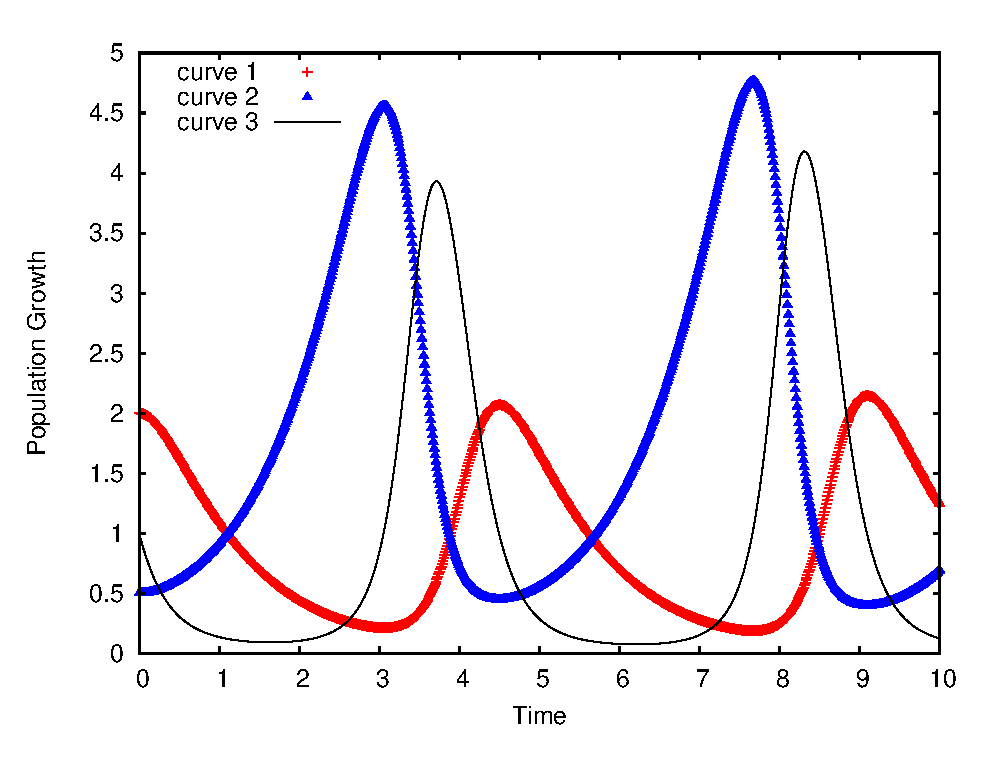
\includegraphics[width=0.85\textwidth]{maxplot.eps} %\caption{}  
      
       Answer:\\
       Curve 2 corresponds x(t), which is prey\\
       Curve 3 corresponds, y(t), which is predator but prey of z(t)\\
       Curve 2 corresponds, z(t).\\  
  \end{figure} 
 % \item Based on the above figure, please sketch a rough phase portrait for populations $xy,$ $yz$
    \item Now assume that the population $x(t)$ in isolation follows the logistic equation. Keeping this assumption in mind, please modify the differential equations obtained in (a) and write the modified system of equations you obtain.
    
    Answer:\\
    \begin{align}
    \frac{dx}{dt} = a_1x(1 - \frac{x}{k}) \\
    \frac{dy}{dt} = -b_1y  -b_3yz\\
    \frac{dz}{dt} = -c_1z + c_2 yz\\
    \end{align}
 \end{enumerate}
%%%%%%%%%%%%%%%  CPS 5401  %%%%%%%%%%%%%%%%%%%%%%%%%%%%%%
%%%%%%%%%%%%%%%%%%%%%%%%%%%%%%%%%%%%%%
\end{enumerate}
\end{document}
